\section{Il problema del tracking nei sistemi AR}
Abbiamo visto che è possibile calcolare la matrice omografica, che permette di convertire un punto tra le coordinate schermo e quelle del mondo reale, ma appena ci spostiamo la matrice omografica non va più bene. 
Il device continua a muoversi e quindi bisogna tenere aggiornata la matrice omografica. Questo è il problema del tracking.

La registration vale quindi per un frame, ma dobbiamo fare la registration per ogni frame?

Vogliamo fare in modo di calcolare una matrice $H^I$ che rappresenti lo spostamento rispetto a quando ho fatto la registrazione $H$ e in modo tale che il prodotto tra le matrici sia la nuova matrice omografica.

Abbiamo 3 possibili soluzioni al problema del tracking:
\begin{enumerate}
    \item registration ripetuta 
    \item tecniche visuo-inerziali
    \item registration e tracking combinate
\end{enumerate}

\subsection{Registration ripetuta}
È la soluzione più semplice, non si fa il tracking e si continua a ripetere la registration. 
È poco efficiente, la registration è complessa e non vogliamo farla ad ogni frame. 
Potrebbe anche non funzionare: prendiamo un marcatore, fino a quando inquadriamo il marcatore possiamo fare la registration, quando non lo inquadriamo più, non la possiamo più fare. 
Dunque, se inquadro il marcatore una volta e poi sposto il device in modo che il marcatore non sia più inquadrato, non riesco ad aggiornare la posizione. In questo caso devo interrompere la sessione AR.

\subsection{Tecniche visuo-inerziali}
Le tecniche visuo-inerziali calcolano lo spostamento (inteso come variazione di posizione e orientamento) e combinano:
\begin{itemize}
    \item tecniche inerziali: sono le stesse tecniche viste nell'indoor positioning. Quando supponiamo che il sistema sia in uno stato di quiete, possiamo calcolare la posizione rispetto alla gravità. Possiamo calcolare quando il device si muove grazie agli accelerometri e quando ruota grazie ai giroscopi.
    Durante gli spostamenti integriamo il valore dei giroscopi e doppio-integriamo quello degli accelerometri per calcolare la posizione rispetto al nostro sistema di riferimento iniziale.
    Queste operazioni di integrazione aumentano l'errore, che causa drift e richiede un frequente fix della posizione
    \item tecniche visuali: è possibile stimare lo spostamento della camera usando tecniche chiamate optical flow. L'idea è quella di cercare di stimare come è stata traslata/ruotata la camera guardando come si sono spostati alcuni punti nell'immagine
\end{itemize}

\subsubsection{Optical flow}
Dato un insieme di punti in un frame al tempo t-1 vogliamo calcolare come questi punti si spostano nel frame successivo al tempo t.
Con punto si intende un pixel o gruppo di pixel di un oggetto del mondo reale.

Ad esempio: supponiamo di avere un'immagine perfettamente bianca, con un solo pixel verde. È molto difficile capire come si sono spostati i pixel bianchi, invece posso facilmente capire come si è spostato il pixel verde. Potrebbero comunque esserci molti casi particolari: ad esempio il pixel verde rappresenta un led che si spegne e un altro led, in posizione differente si accende.

Quali punti consideriamo?
\begin{itemize}
    \item Approcci “dense”: tutti i punti dell'immagine
    \item Approcci “sparse”: solo per alcuni punti caratteristici (es: feature points)
\end{itemize}

In linea teorica, il problema non è risolvibile, perché non sappiamo nulla di come cambiano i punti tra un'immagine e l'altra, ad esempio potrebbe cambiare l'intensità per via dell'illuminazione.
Ciascun punto potrebbe spostarsi in qualunque punto dell'immagine o anche sparire fuori dall'immagine al tempo t, così come al tempo t potrebbero apparire dei punti che non erano inquadrati al tempo t-1. 

In realtà si possono fare alcune assunzioni che rendono il problema risolvibile, in modo efficace, in molti casi pratici:
\begin{itemize}
    \item small motion: i punti non si muovono molto lontano
    \item brightness constancy: le forme rimangono (più o meno) simili
    \item spatial coherence: i punti si muovono più o meno come i loro vicini
\end{itemize}

Presi due frame a distanza molto ravvicinata, queste assunzioni sembrano ragionevoli, almeno in molti casi. 
Anche basandosi su queste assunzioni la soluzione del problema dell'optical flow non è banale.

La tecnica è ancora più efficiente se viene adottata su un insieme limitato di punti, per esempio si può adottare per i feature points, già identificati per la registrazione markerless. Non calcoliamo lo spostamento per tutti i punti dell'immagine ma solo per alcuni.

Le tecniche inerziali e visuali possono essere combinate, per realizzare una sistema maggiormente robusto, con tecniche come filtri di Kalman o particle filtering. 
Le librerie di AR esistenti adottano tecniche di calcolo dello spostamento visuo-inerziali.
Queste tecniche risolvono il problema del marcatore con la registration: se non inquadro il marcatore riesco a calcolare la matrice omografica. 
 
\subsection{Registration e tracking combinate}
Se faccio la registrazione una volta e poi continuo ad usare tecniche visuo inerziali, l'errore viene sempre più accumulato. Nei sistemi di AR questo significa che gli oggetti virtuali mostrati a schermo non sono solidali con l'ambiente.

Per risolvere il problema, concettualmente vorremmo avere un modo per azzerare il drift periodicamente. 
Quando usiamo tecniche markerless, troviamo la posizione della camera rispetto a certi oggetti (landmark) caratteristici dell'ambiente, ma questo non ci permette di fare un fix di posizione, perché non sappiamo dove sono quegli oggetti. 

Se noi inquadriamo un landmark, poi ci spostiamo e poi ritorniamo ad inquadrarlo, possiamo usare quello stesso landmark come fix di posizione.
Queste operazioni di registration e tracking diventano parte intergrante di un'unica tecnica che si chiama SLAM (simultaneous localization and mapping). 

\subsubsection{Esempio SLAM}
Supponiamo di girare attorno ad un edificio e mentre lo facciamo, identifichiamo i feature points. L'edificio è rettangolare, ma il sistema visuo-inerziale sta sbagliando: ha calcolato gli angoli in modo errato e dunque il rettangolo non si chiude.

Se però riusciamo ad accorgerci che siamo tornati nello stesso punto della partenza (perché riconosciamo gli stessi feature points) possiamo correggere l'errore, non solo nella posizione corrente, ma anche in tutte quelle precedenti.

\begin{figure}[!ht]
\begin{center}
    \fbox{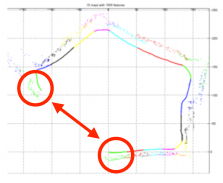
\includegraphics[width=.4\textwidth]{images/MobiDEV/2. tecniche di aggregazione di dati soggetti a rumore/slam1.PNG}}
    \qquad \fbox{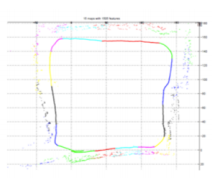
\includegraphics[width=.4\textwidth]{images/MobiDEV/2. tecniche di aggregazione di dati soggetti a rumore/slam2.PNG}}
\end{center}

\end{figure}
